%% Document template source: LaTeX2e template for FEUP's Project FE-UP
%% Document template author: jlopes@fe.up.pt
%% Template adapted

%% A alterar: <--ALTERAR-->

\documentclass[11pt,a4paper]{report}

%% Macros ----------------------------------------------------------------------
\newcommand{\school}{Instituto Superior de Engenharia de Lisboa}
\newcommand{\degree}{Licenciatura em Engenharia Eletrotécnica, Telecomunicações e Computadores}
\newcommand{\projisel}{Projeto ISEL 2023/24 --- LEETC}
\newcommand{\projtitle}{Computer Networks}
\newcommand{\projsubtitle}{Phase 1 - Web Server}
\newcommand{\projteam}{Grupo LP-07}

%% Package ---------------------------------------------------------------------
\usepackage{graphicx}           % 
\usepackage[english]{babel}     % [portuges]??
\usepackage{multicol}           % 
\usepackage{longtable}          % Tables continue in the next page
\usepackage{listings}           % Programming syntax
\usepackage{array}              % Images in tables
\usepackage[export]{adjustbox}

\usepackage[utf8]{inputenc}     % accents
\usepackage{color}
\usepackage{lastpage}           % 
\usepackage{fancyhdr}           % Headers and footers
\usepackage{hyperref}           % Hyper references
\usepackage{chicago}            % Bibliography style
\usepackage{caption}              % rotating captions, sideways captions, etc.
\usepackage{subcaption}           % for subfigures and the like
\usepackage{float}                % tables and figures in the multi-column environment 
\usepackage[a4paper,left=25mm,right=25mm,top=25mm,bottom=25mm,headheight=6mm,footskip=12mm]{geometry}   % Document dimensions

%verificar
\usepackage[T1]{fontenc}          % PS fonts
\usepackage{newtxtext,newtxmath}  % do not use CM fonts
\usepackage{amsmath}              % multi-line and other mathematical statements
\usepackage{setspace}             % setting the spacing between lines
\usepackage[normalem]{ulem}       % various types of underlining
\usepackage{multirow}             % tabular cells spanning multiple rows
\usepackage[table]{xcolor}        % driver-independent color extensions
\usepackage{lipsum}               % loren dummy text
%\setlength{\marginparwidth}{2cm}  % todonotes' requirements
%\usepackage{todonotes}            % todo's

%% my other macros, if needed
\newcommand{\windspt}{\textsf{WindsPT\/}}
\newcommand{\windscannerpt}{\emph{Windscanner.PT\/}}
\newcommand{\class}[1]{{\normalfont\slshape #1\/}}
\newcommand{\svg}{\class{SVG}}

%% my environments for infos
\newenvironment{info}[1]{\vspace*{6mm}\color{blue}[ \begin{em} #1}
                        {\vspace*{6mm}\end{em} ]}
\newenvironment{infoopt}[1]{\vspace*{6mm}\color{blue}[ \textbf{Elemento opcional.} \begin{em} #1}
                        {\vspace*{6mm}\end{em} ]}

%% Package settings ------------------------------------------------------------
\graphicspath{{./images/}}                          % {graphicx} - Images path
\selectlanguage{portuguese}                         % {babel} - Language portuguese
\setlength{\columnsep}{3cm}                         % {multicol} - Column spacement
\definecolor{engineering}{rgb}{0.549,0.176,0.098}   % {color}
\definecolor{cloudwhite}{cmyk}{0,0,0,0.025}         % {color}
\definecolor{deepblue}{rgb}{0,0,0.5}
\definecolor{deepred}{rgb}{0.6,0,0}
\definecolor{deepgreen}{rgb}{0,0.5,0}
\setlength{\parindent}{0em}                         % {geometry}
\setlength{\parskip}{1ex}                           % {geometry}
\lstdefinestyle{pythoncode}                         % {listings} - Python syntax
{
    keepspaces=true,
    numbersep=5pt,
    basicstyle=\footnotesize\ttfamily,
    keywordstyle=\bfseries\color{deepblue},
    stringstyle=\color{deepgreen},
    numbers=left,                                   % where to put the line-numbers
    numberstyle=\scriptsize\texttt,                 % the size of the fonts that are used for the line-numbers
    stepnumber=1,                                   % the step between two line-numbers. If it's 1 each line will be numbered
    numbersep=8pt,                                  % how far the line-numbers are from the code
    frame=tb,
    float=htb,
    aboveskip=8mm,
    belowskip=4mm,
    backgroundcolor=\color{cloudwhite},             
    showspaces=false,                               % show spaces adding particular underscores
    showstringspaces=false,                         % underline spaces within strings
    showtabs=false,                                 % show tabs within strings adding particular underscores
    tabsize=2,                                      % sets default tabsize to 2 spaces
    captionpos=b,                                   % sets the caption-position to bottom
    breaklines=true,                                % sets automatic line breaking
    breakatwhitespace=false,                        % sets if automatic breaks should only happen at whitespace
    escapeinside={\%*}{*)},                         % if you want to add a comment within your code
    morekeywords={*,var,template,new}               % if you want to add more keywords to the set
}
\fancyhf{}                                          % {fancyhdr} clear off all default fancyhdr headers and footers
\lfoot{\small{\emph{\projtitle, \projsubtitle}}}    % {fancyhdr}
\rfoot{\small{\thepage\ / \pageref{LastPage}}}      % {fancyhdr}
\pagestyle{fancy}                                   % {fancyhdr} apply the fancy header style
\renewcommand{\headrulewidth}{0.0pt}                % {fancyhdr} no head rule
\renewcommand{\footrulewidth}{0.4pt}                % {fancyhdr}
\hypersetup{                                        % {hyperref}
    plainpages=false,
    pdfpagelayout=SinglePage,
    bookmarksopen=false,
    bookmarksnumbered=true,
    breaklinks=true,
    linktocpage,
    colorlinks=true,
    linkcolor=engineering,
    urlcolor=engineering,
    filecolor=engineering,
    citecolor=engineering,
    allcolors=engineering
}

%\usepackage{comment}               % Permite criar um segmento de comentários (/begin{comment} [...] /end{comment})
%\usepackage{fullpage}              % Utilizar página inteira

%% Document start --------------------------------------------------------------
\begin{document}
\pagenumbering{roman}\setcounter{page}{1}

%% Cover -----------------------------------------------------------------------
\begin{titlepage}
    \center

    \vspace*{-12mm}
    {\large \textbf{\textsc{\school}}}\\

    \vfill

    
\includegraphics[width=62mm]{logoisel}
    
    \vfill
    
    {\huge \textbf{\projtitle}}\\[6mm]
    {\Large \textbf{\projsubtitle}}\\
    
    \vfill
    
    \vfill
    
    {\Large \textbf{\projisel}}\\[12mm]
    
    {\Large \textbf{Coordination}}\\[4mm]
    {\large General: Carlos Meneses\hspace*{18mm}
            Course: Nuno Cruz}\\[6mm]
    
    {\Large \textbf{\projteam}}\\[4mm]
    {\large Supervisor: Luís Pires\hspace*{12mm}}\\[6mm]
    
    {\Large \textbf{Student}}\\[4mm]
    {\large Nuno Brito $<$A46948@alunos.isel.pt$>$}
    
    \vspace*{10mm}
    
    \renewcommand{\today}{April 14th 2024}
    \today
    
\end{titlepage}

%% TOC -------------------------------------------------------------------------{{{1
\tableofcontents

%% List of figures -------------------------------------------------------------{{{1
\listoffigures
\addcontentsline{toc}{chapter}{Figure list}

%% List of tables --------------------------------------------------------------{{{1
\listoftables
\addcontentsline{toc}{chapter}{Table list}

%% List of listings --------------------------------------------------------------{{{1
\lstlistoflistings
\addcontentsline{toc}{chapter}{Listings list}

%% Acronyms --------------------------------------------------------------------{{{1
\chapter*{Acronyms list}
    \addcontentsline{toc}{chapter}{Acronyms list}

    \begin{flushleft}
        \begin{tabular}{l p{0.8\linewidth}}
            API     & Application Programming Interface\\
            GUI     & Graphical User Interface\\
            HTTP    & Hyper Text Transfer Protocol\\
            HTTPS   & Hyper Text Transfer Protocol Secure\\
            OS      & Operating System\\
            OSS     & openSUSE\\
            PHP     & PHP: Hypertext Preprocessor\\
            SSL     & Secure Sockets Layer\\
            TCP     & Transmission Control Protocol\\
            TLS     & Transport Layer Security\\
            TUI     & Terminal User Interface\\ % Not used yet
            UDP     & User Datagram Protocol\\
            VPN     & Virtual Private Network\\
            WWW     & World Wide Web\\
            XAMPP   & Cross-Platform, Apache, MySQL, PHP, and Perl
        \end{tabular}
    \end{flushleft}

%% Glossary --------------------------------------------------------------------{{{1
\chapter*{Glossary}
    \addcontentsline{toc}{chapter}{Glossary}

    \begin{description}
        \item[Operating system] \hfill \\
            A program that manages a computer's resources from software to hardware.
        \item[Browser] \hfill \\
            A browser is a internet navigation software. It comes in multiple flavours, nowadays the big three are Microsoft Edge, Mozilla Firefox and Google Chrome.
        \item[Windows] \hfill \\
            Microsoft's operating system. First released in 1985 as a Graphical User Interface (GUI) for MS-DOS, continued to evolve with it's latest version being 11.
        \item[Rolling release distribuition] \hfill \\
            A distribuition where it's software release cycle is more frequent than those of Long Term Support (LTS). It's up to the Linux-based distribuitor to guarantee the testing of a package.
            Due to it's nature, it's not recommended for server production environment.
        \item[openSUSE Tumbleweed] \hfill \\
            An openSUSE (OSS) is an open-source community driven Linux-based distribuition sponsored by SUSE Software Solutions. Tumbleweed is a rolling release version allowing for up-to-date software releases.
        \item[Wireshark] \hfill \\
            Wireshark is a network protocol analyser software. Allows traffic capture between a computer and a network.
        \item[LibreWolf] \hfill \\
            An internet browser based on Mozilla's Firefox. It's primary purpose is to allow privacy, and with it comes security. It achieves this by removing telemetry and data collection.
        \item[XAMPP] \hfill \\
            A software package environment collection containing Apache2 webserver, MariaDB database, PHP and Perl.
        \item[Apache2] \hfill \\
            An opensource HTTP web server.
        \item[MariaDB] \hfill \\
            A community-developed fork of MySQL database server.
        \item[Perl] \hfill \\
            A high-level, general-purpose, interpreted, dynamic programming language
        \item[Socket] \hfill \\
            A network socket serves as an endpoint for sending and receiving data across the network.
        \item[Python] \hfill \\
            Python is a high-level programming language, object-oriented.
        \item[Firewall] \hfill \\
            A barrier between networks. Controls inbound and outbound traffic.
        \item[VPN] \hfill \\
            A private network creating a secure connection between a device and a network.
    \end{description}

%% Chapter: introduction -------------------------------------------------------{{{1
\chapter{Introduction}
%% display headers & footers
\pagestyle{fancy}
The project consists in building a computer network through four phases. First with a webserver, then simulating a local area network (LAN) with two computers and a switch.
By the end of the journey, this project will develop into something similar to a corporate network.

%% main page numbers with arabic numerals
\pagenumbering{arabic}\setcounter{page}{1}

%% Chapter: project ------------------------------------------------------------{{{1
\chapter{Phase 1}
    \section{Milestones}
        \begin{itemize}
            \item Setup apache2 web server in localhost
            \item Access web server locally (http://127.0.0.1/ or http://localhost)
            \item Access web server from a remote computer (http://172.24.1.12)
            \item Use wireshark in a remote host to capture packages from the server
            \item Compare the HTTP headers sent by the client and the server
            \item Develop a simple barebones HTTP webclient
            \item Establish a TCP connection to the server
            \item Request the base webpage
        \end{itemize}
        
    \section{WebClient requirements}
        \begin{itemize}
            \item HTTP library forbidden
            \item Establish TCP connection using available sockets library - send/receive the HTTP request/reply
            \item Output HTTP reply to the user
            \item - Optional - act to the various HTTP replies
            \item Text-only application
        \end{itemize}

    \section{Software}
        \begin{itemize}
            \item Local server side
                \subitem Operating system: Windows 11 x64
                \subitem WebServer: XAMPP x64 8.2.12-0-VS16 for windows
            \item Client side
                \subitem Operating system: openSUSE Tumbleweed
                \subitem Browser: LibreWolf version 123.0-1
                \subitem Package monitor: Wireshark version 4.2.3 (Git commit b0da86c196d1).
        \end{itemize}

    \section{Software install}
        \begin{flushleft}
            First we install, start and configure XAMPP. Using the following link, \href{https://www.apachefriends.org/download.html}{https://www.apachefriends.org/download.html}, we can choose our prefered method, for this project the portable version was the best choice since no installation was needed. After uncompressing our downloaded file, we can start the process.
                \begin{center}
                    \begin{longtable}{ m{5cm} l }
                        \textbf{Steps} & \textbf{Example} \\
                        \hline
                        \endfirsthead
                        {{\bfseries \tablename\ \thetable{} -- continued}} \\
                        \textbf{Steps} & \textbf{Example} \\
                        \hline
                        \endhead
                        \hline Continued on next page \\
                        \endfoot
                        \endlastfoot

                        The read me file available in the root directory states that we need to run \textit{setup\_xampp} batch file first to populate the registry it's directory.
                        & 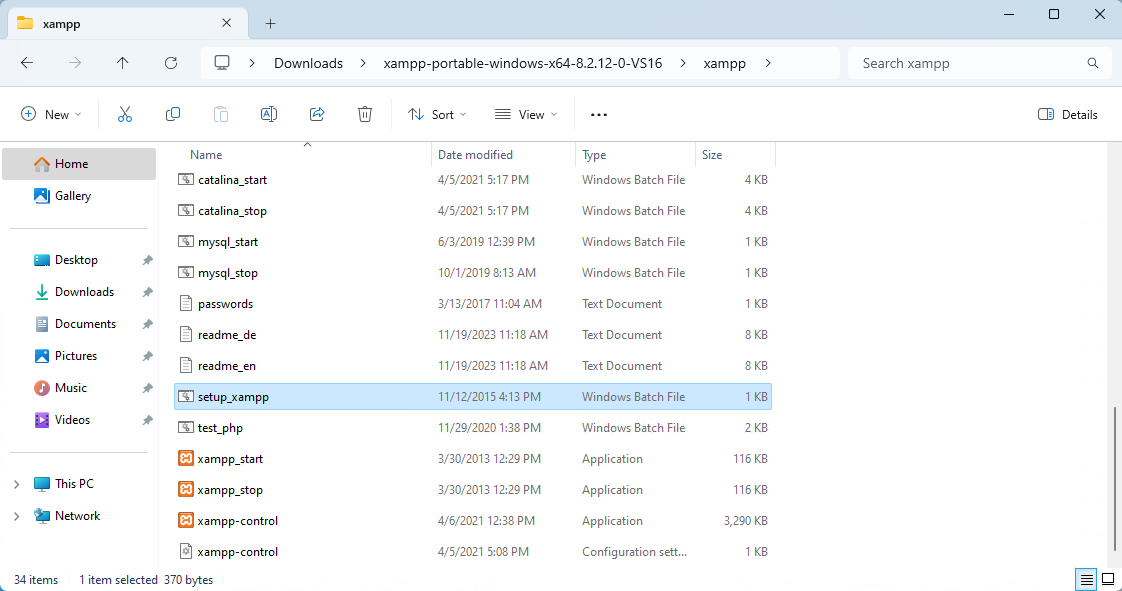
\includegraphics[scale=0.35,valign=c]{install_xampp08} \\
                        \hline
                        
                        After completing, just press any button to continue.
                        & 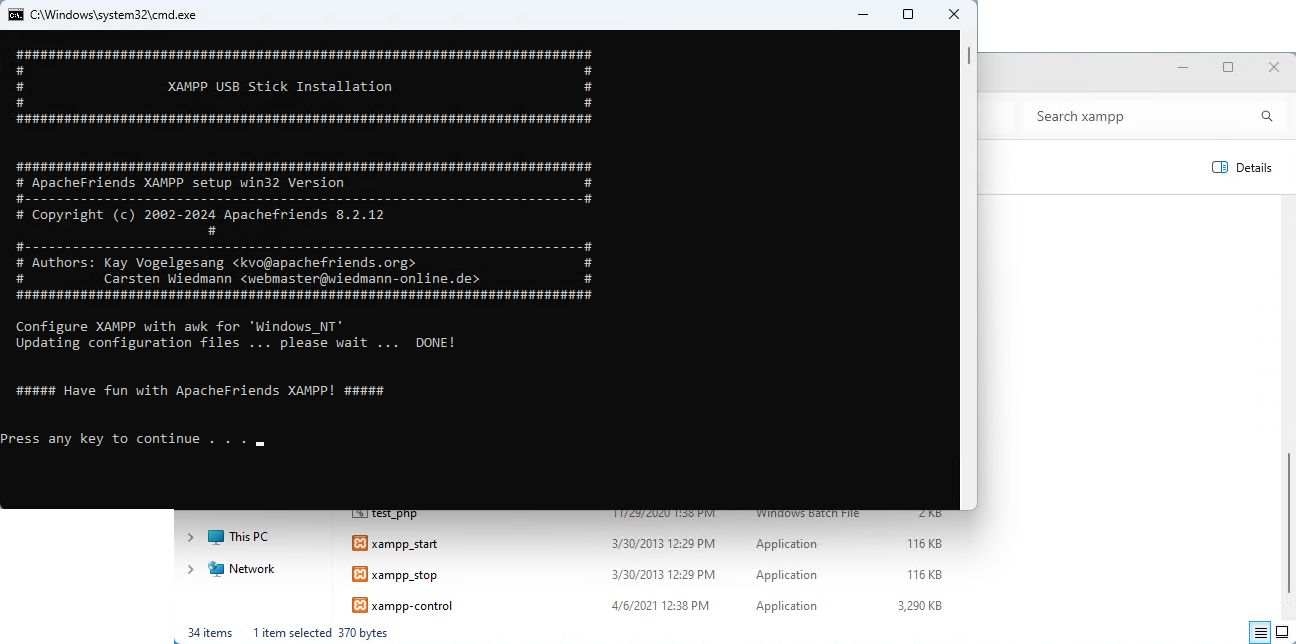
\includegraphics[scale=0.303,valign=c]{install_xampp09} \\
                        \hline
                        
                        Next click in the \textit{xampp\_start} executable, windows will prompt some firewall permissions which will gladly accept.
                        & 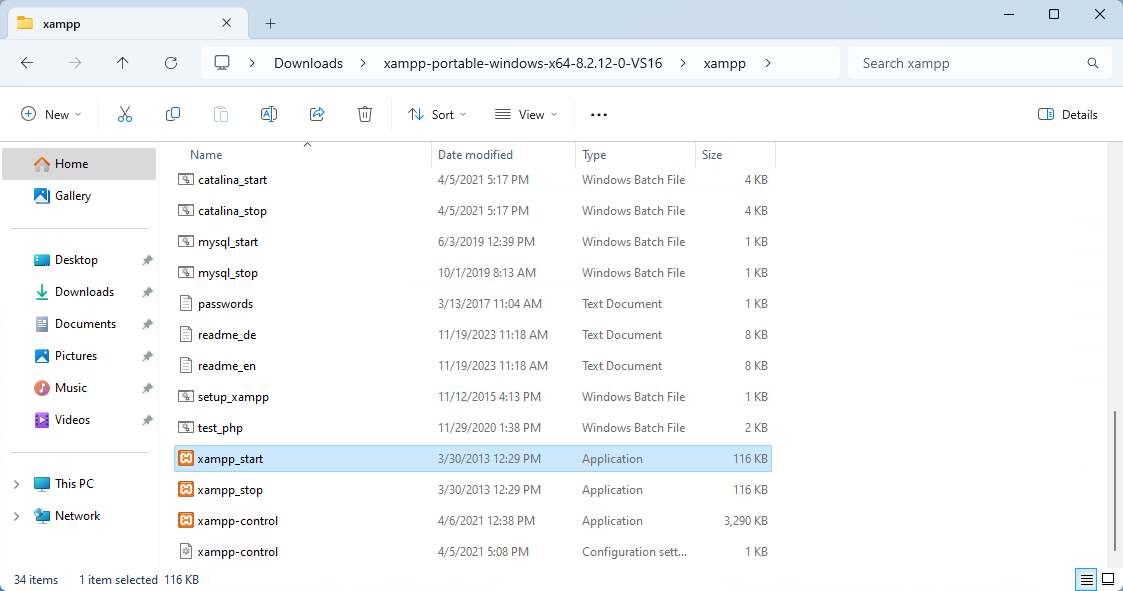
\includegraphics[scale=0.35,valign=c]{install_xampp10} \\
                        & 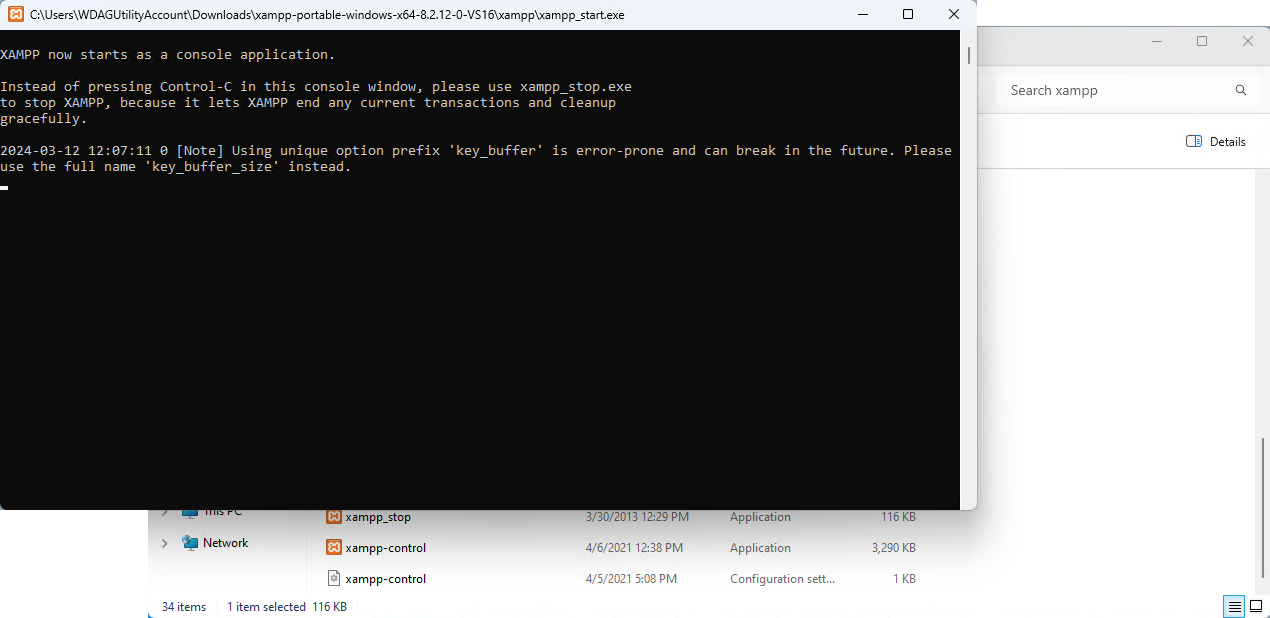
\includegraphics[scale=0.303,valign=c]{install_xampp13} \\
                        \hline
                        
                        Pick a language for the program.
                        & 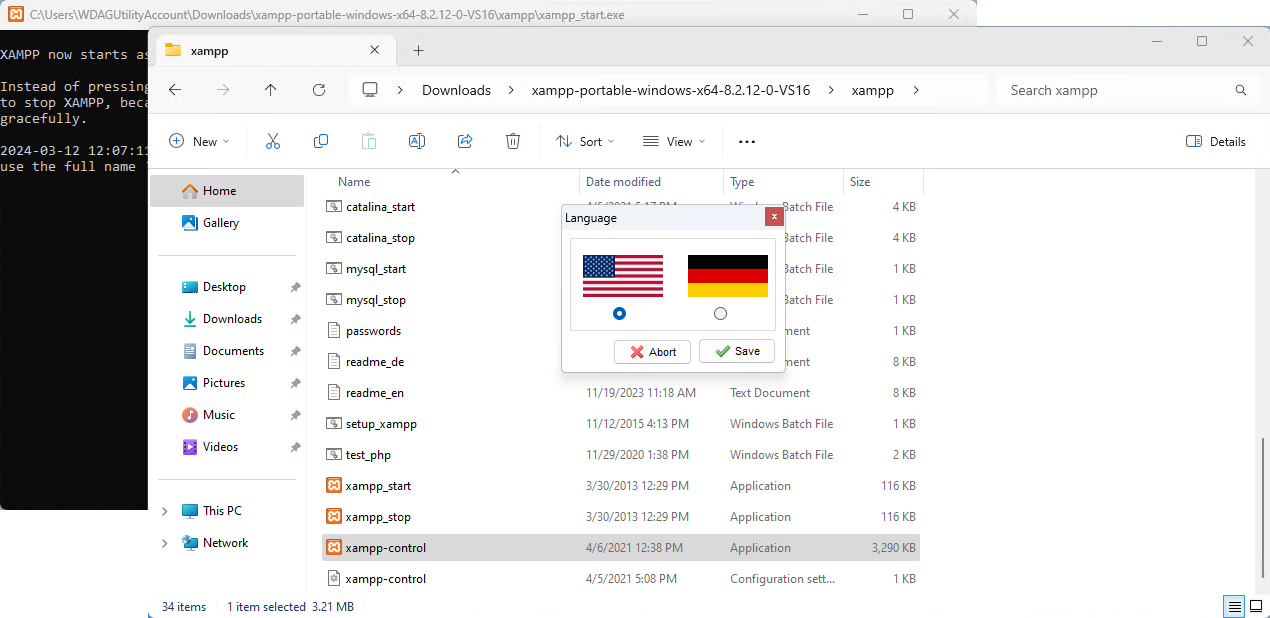
\includegraphics[scale=0.303,valign=c]{install_xampp14} \\
                        \hline
                        
                        Apache2 comes with SSL on by default. Since we're studying the HTTP protocol it's convenient to disable HTTPS. Pressing the \textit{config} button shows a list of configuration files. Select \textit{Apache (httpd-ssl.conf)}.
                        & 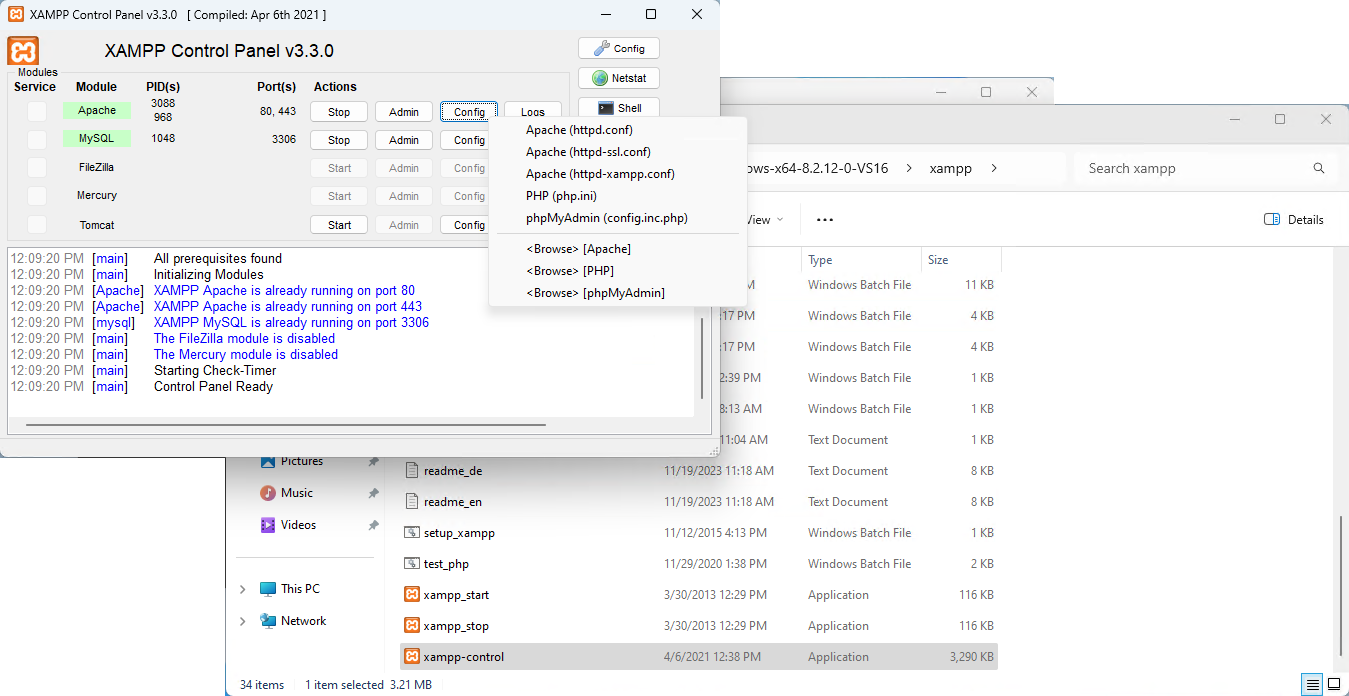
\includegraphics[scale=0.285,valign=c]{install_xampp15} \\
                        \hline
                        
                        Search and comment the line with \textit{SSLEngine on}.
                        & 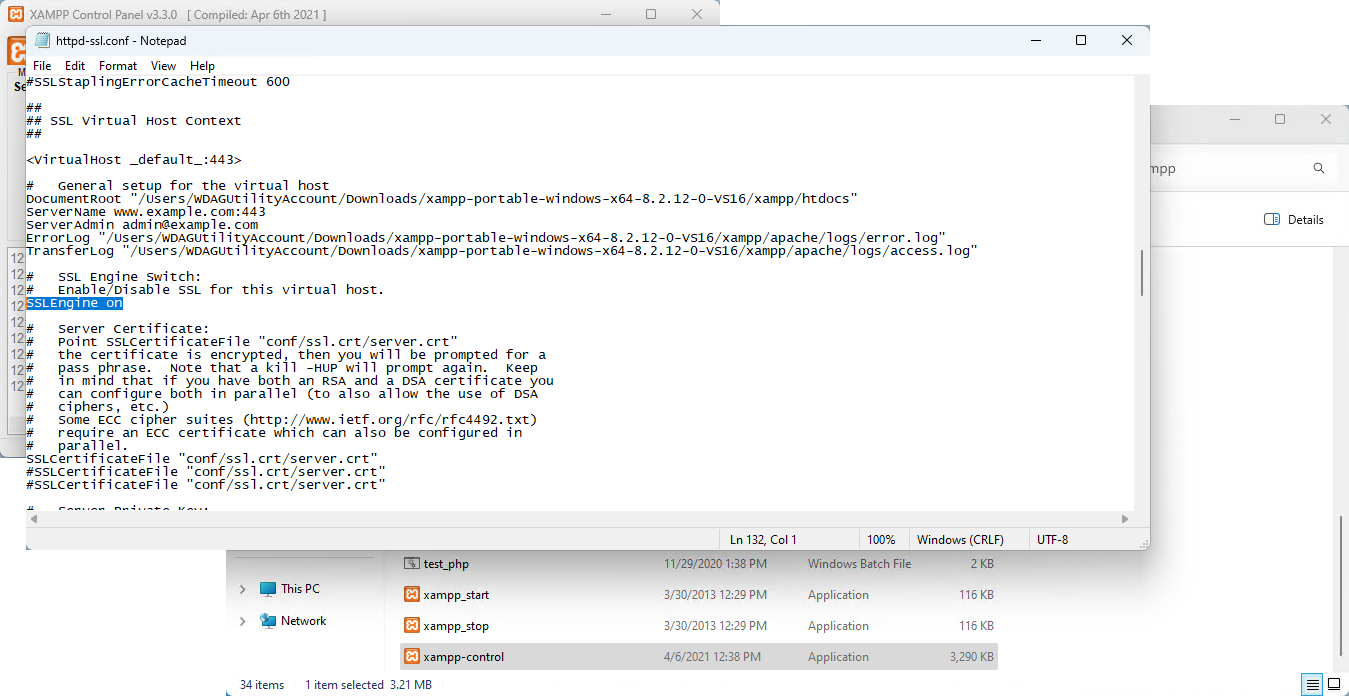
\includegraphics[scale=0.285,valign=c]{install_xampp16} \\
                        \hline
                        
                        \begin{flushleft}
                            Previously if we went to \textit{http://localhost} it would redirect to the HTTPS version. After completing the above step it'll no longer redirect, showing us the non-secure version.
                        \end{flushleft}
                        & 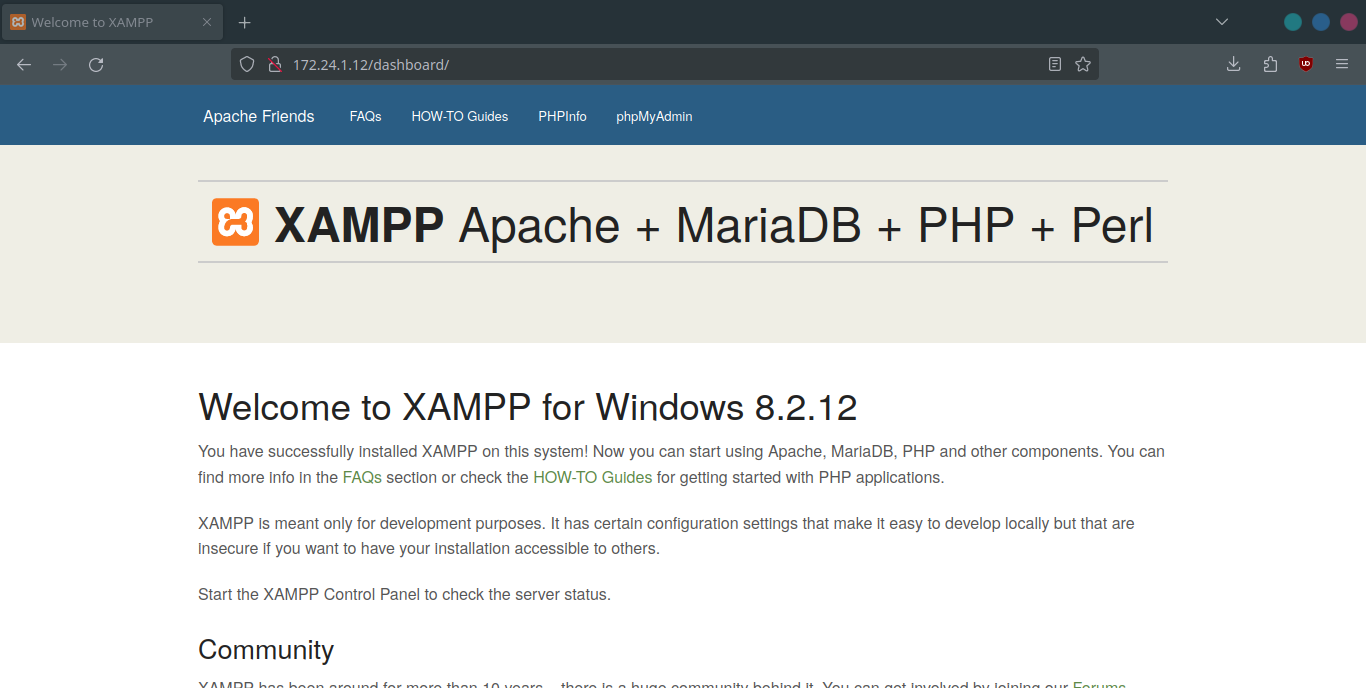
\includegraphics[scale=0.285,valign=c]{install_xampp17} \\
                        \hline

                        \caption{XAMPP install} \label{tab:xampp}
                    \end{longtable}
                \end{center}

            Next up is wireshark, the powerful network analyser. We'll download the installer from \href{https://www.wireshark.org/download.html}{https://www.wireshark.org/download.html}.
                \begin{center}
                    \begin{longtable}{ m{5cm} l }
                        \textbf{Steps} & \textbf{Example} \\
                        \hline
                        \endfirsthead
                        {{\bfseries \tablename\ \thetable{} -- continued}} \\
                        \textbf{Steps} & \textbf{Example} \\
                        \hline
                        \endhead
                        \hline Continued on next page \\
                        \endfoot
                        \endlastfoot

                        Wireshark setup. Select everything available and continue by clicking \textit{next}.
                        & 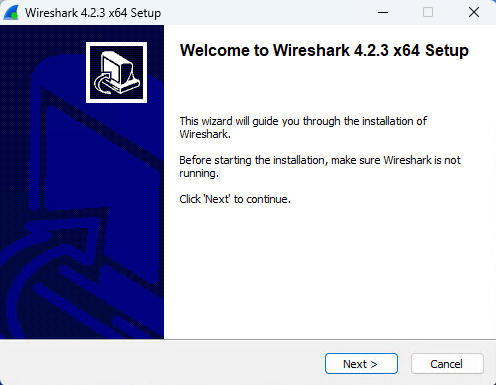
\includegraphics[scale=0.80,valign=c]{install_wireshark02} \\
                        \hline
                        After completing the installation, reboot the computer.
                        & 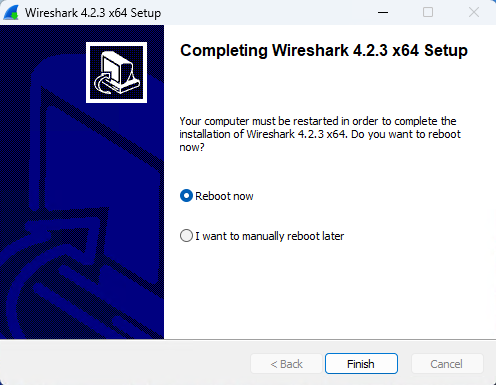
\includegraphics[scale=0.80,valign=c]{install_wireshark21} \\
                        \hline

                        \caption{Wireshark install} \label{tab:wireshark}
                    \end{longtable}
                \end{center}
        \end{flushleft}

    \section{WebClient - Python Code}
        \lstset{style=pythoncode}
        \lstinputlisting[
            language=python,
            caption={Simple HTTP WebClient using sockets in python},
            label={lst:webclientpy}
        ]{webclient/httpsocketv3.py}
        
        \begin{flushleft}
            The code listed in \ref{lst:webclientpy} was adapted to be simple and cycle through the various request messages without any user input. \\
            Modifiable variables include \textit{serverName}, \textit{serverPort} and the \textit{httpTestMessages} list. \\
        \end{flushleft}

        The webclient produces the following output:
        \lstinputlisting[
            language={},
            caption={WebClient output},
            label={lst:webclientoutput}
        ]{./webclient/httpsocketv3output20240329.txt}

    \section{Wireshark captures}
        \begin{flushleft}
            First we must ensure the browser being used can connect to the XAMPP server with HTTP. We can do that by enabling the usage of deprecated TLS.
            \clearpage
            \begin{figure}[h]
                \centering
                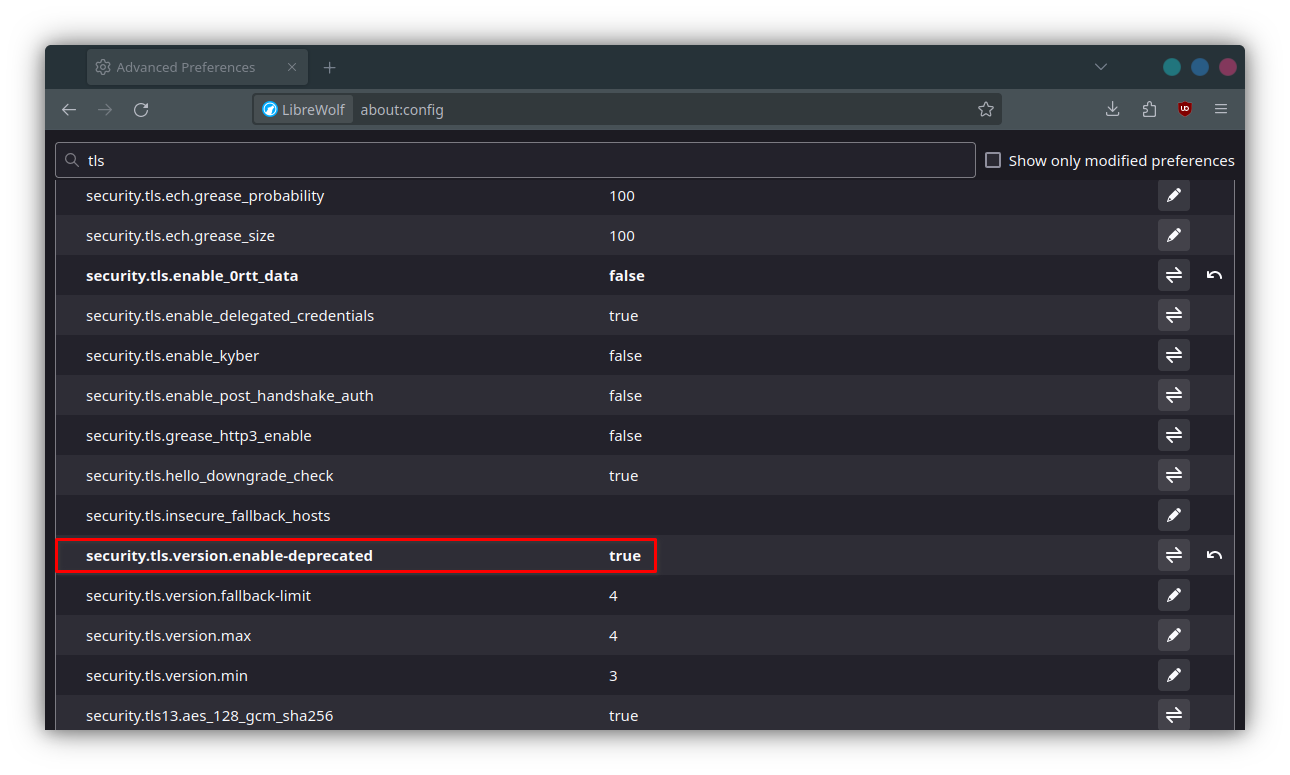
\includegraphics[scale=0.4]{librewolf_tls} 
                \caption{Changing from false to true the \textit{security.tls.version.enable-deprecated} option}
                \label{fig:librewolf}
            \end{figure}

            Then we can start our capture process, next follows some printscreen examples filtered by HTTP.
            \begin{flushleft}
                \begin{figure}[h]
                    \centering
                    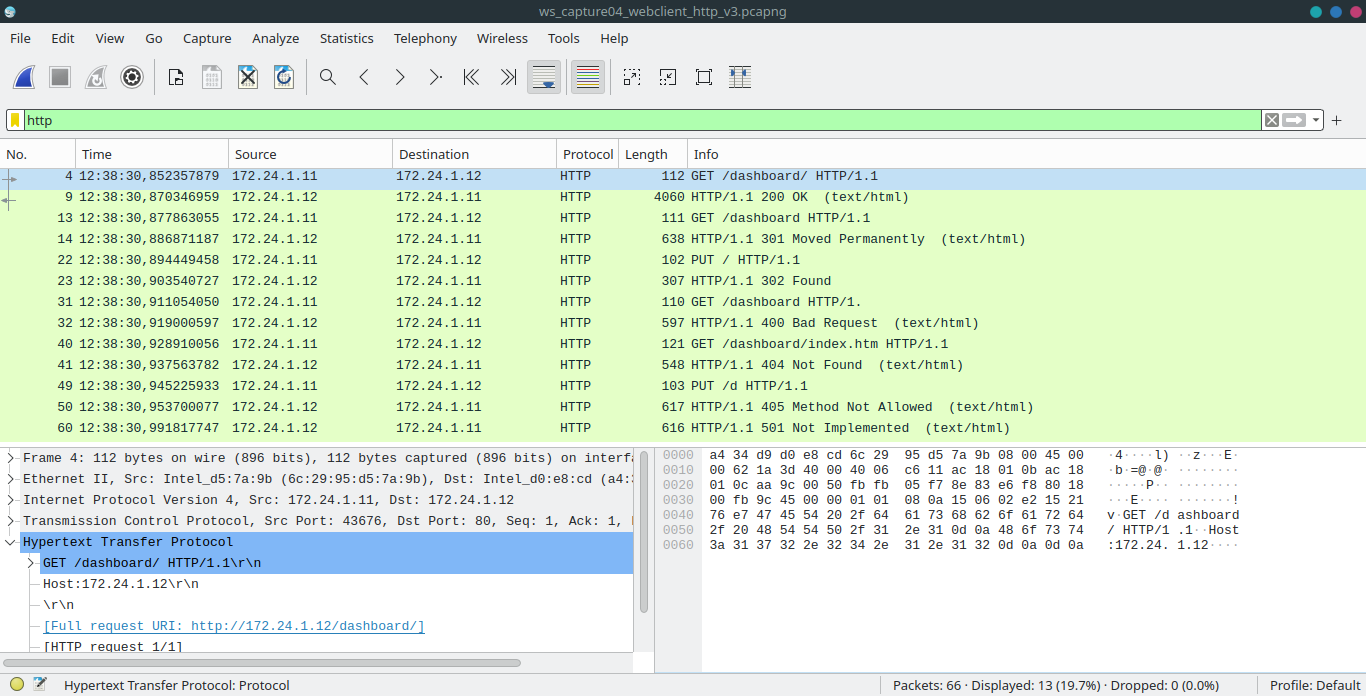
\includegraphics[scale=0.43]{wscapwcsocket05} % Webclient get
                    \caption{Webclient get capture} \label{fig:wireshark1}
                \end{figure}
                
                \begin{figure}[t]
                    \centering
                        \begin{subfigure}{0.49\linewidth} \centering
                            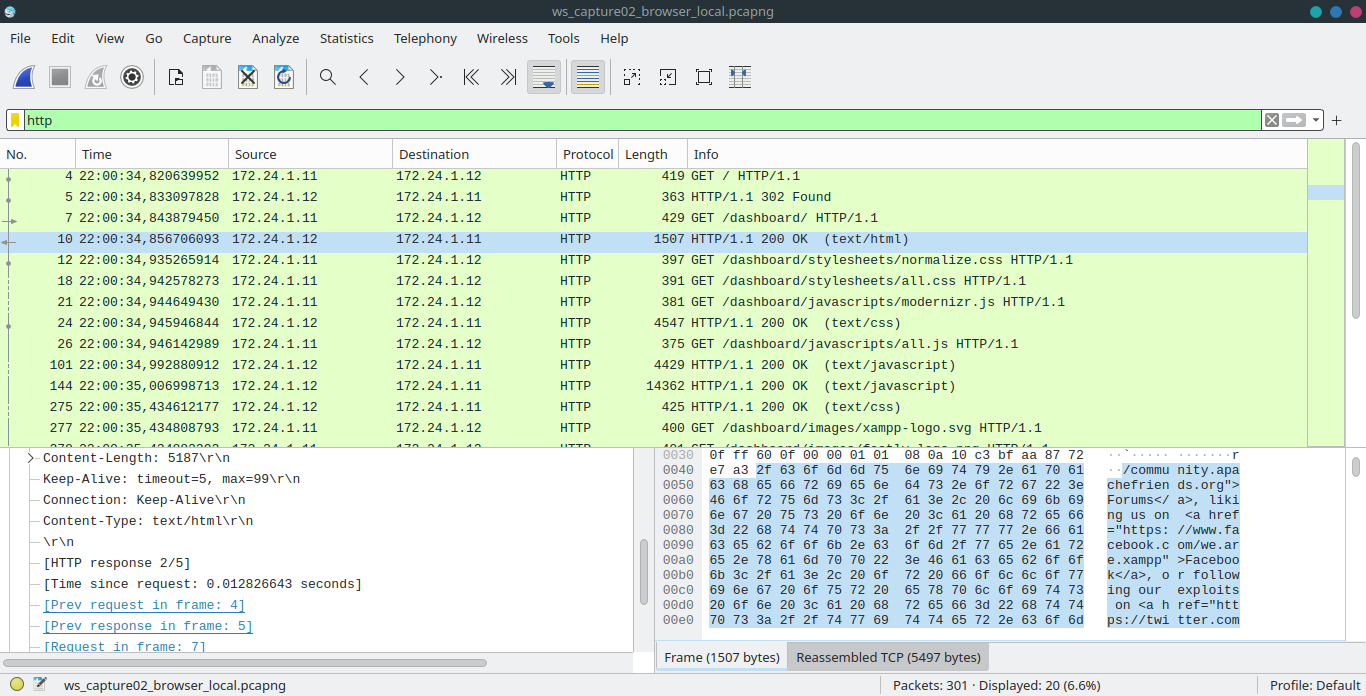
\includegraphics[scale=0.20]{wscapwcsocket08} % Browser local
                            \caption{Browser} \label{fig:wireshark4}
                        \end{subfigure}
                        \begin{subfigure}{0.49\linewidth} \centering
                            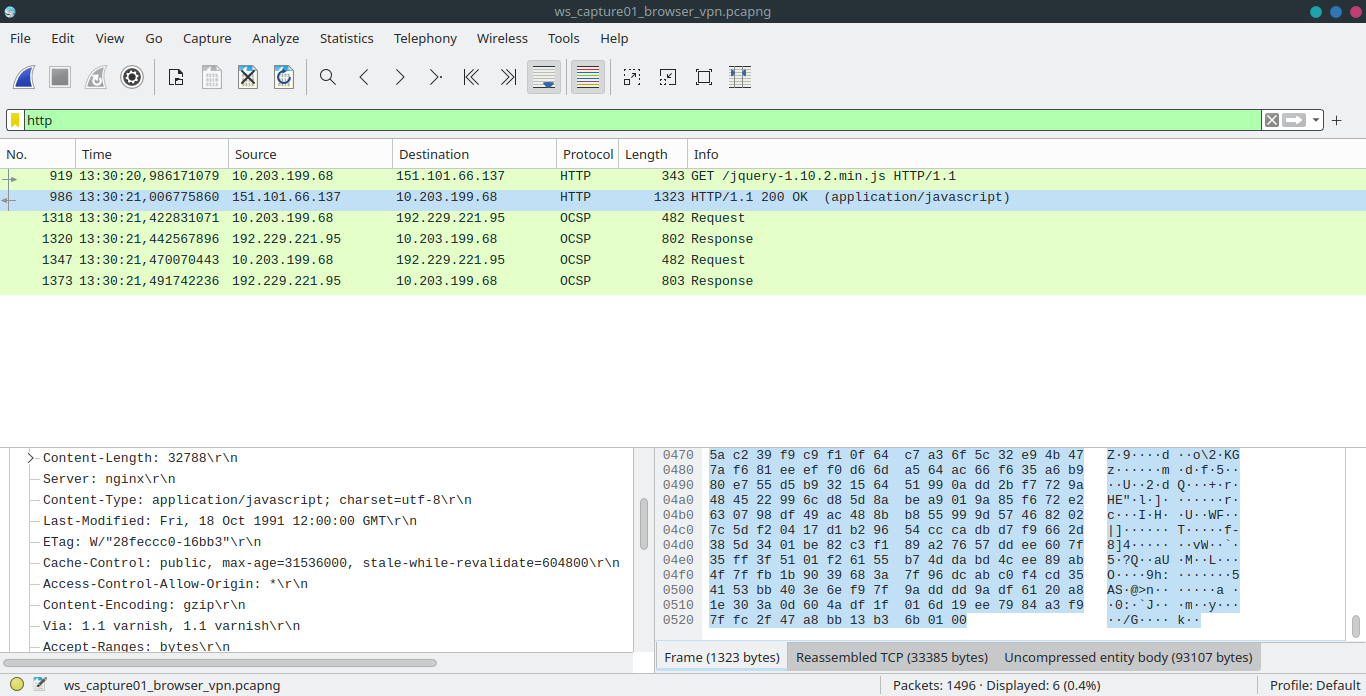
\includegraphics[scale=0.20]{wscapwcsocket07} % Browser vpn
                            \caption{Browser (VPN)} \label{fig:wireshark3}
                        \end{subfigure}
                    \caption{Browser capture} \label{fig:twobrowsers}
                    \end{figure}

                \begin{figure}
                    \centering
                    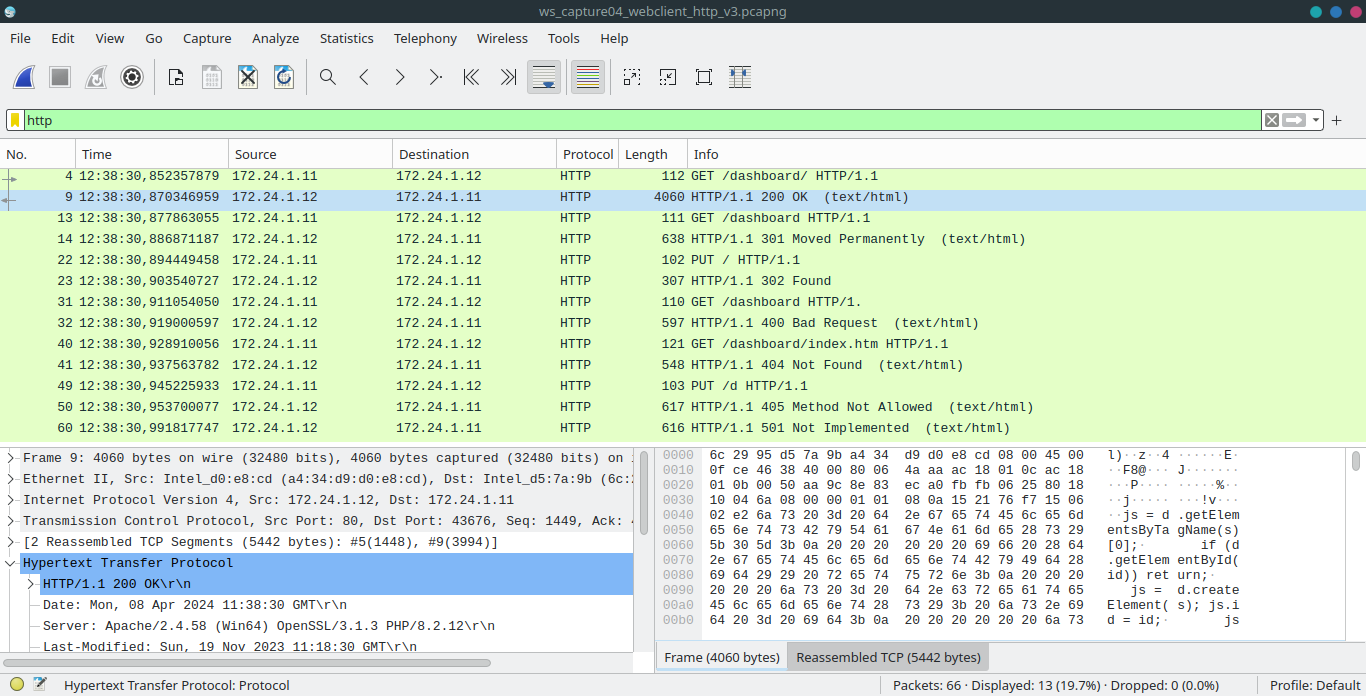
\includegraphics[scale=0.43]{wscapwcsocket06} % Webclient reply
                    \caption{Webclient reply capture} \label{fig:wireshark2}
                \end{figure}
            \end{flushleft}
            
            \clearpage
            To compliment the images, below are segmented outputs (the important parts):
            \lstinputlisting[
                language={},
                %firstline=1,
                %lastline=2,
                linerange={1-2,
                            108-127,
                            129-130,
                            247-284},
                caption={Wireshark capture output sample - VPN},
                label={lst:wiresharkoutvpn}
            ]{./wireshark/wscapture01export.txt} % vpn
            \lstinputlisting[
                language={},
                linerange={1-2,
                            108-130,
                            132-133,
                            241-266},
                caption={Wireshark capture output sample - Browser},
                label={lst:wiresharkoutbrowser}
            ]{./wireshark/wscapture02export.txt} % browser
            \lstinputlisting[
                language={},
                linerange={1-2,
                            8-6,
                            16-17,
                            24-39},
                caption={Wireshark capture output sample - WebClient},
                label={lst:wiresharkoutwebclient}
            ]{./wireshark/wscapture04export.txt} % webclient
        \end{flushleft}

    \section{List of headers and replies}
        \textbf{Request:} GET /dashboard/ HTTP/1.1\textbackslash r\textbackslash nHost:127.24.1.12 \textbackslash r\textbackslash n\textbackslash r\textbackslash n \\
        \textbf{Reply:} HTTP/1.1 200 OK \\
        Meaning: this header complies with what the server expects from a webclient request. \\
        \\
        \textbf{Request:} GET /dashboard HTTP/1.1\textbackslash r\textbackslash nHost:127.24.1.12 \textbackslash r\textbackslash n\textbackslash r\textbackslash n \\
        \textbf{Reply:} HTTP/1.1 301 Moved Permanently \\
        Meaning: this header request a relative directory without a forward slash at the end, prompting the server to reply with a "moved" answer. \\
        \\
        \textbf{Request:} PUT / HTTP/1.1\textbackslash r\textbackslash nHost:127.24.1.12 \textbackslash r\textbackslash n\textbackslash r\textbackslash n \\
        \textbf{Reply:} HTTP/1.1 302 Found \\
        Meaning: this header request is an upload request to an unexistent directory. \\
        \\
        \textbf{Request:} GET /dashboard HTTP/1.\textbackslash r\textbackslash nHost:127.24.1.12 \textbackslash r\textbackslash n\textbackslash r\textbackslash n \\
        \textbf{Reply:} HTTP/1.1 400 Bad Request \\
        Meaning: this header request, although it has an invalid directory, has the HTTP protocol version badly writen (HTTP/1.1 vs. actual HTTP/1.) which causes a "bad request" reply from the server. \\
        \\
        \textbf{Request:} GET /dashboard/index.htm HTTP/1.1\textbackslash r\textbackslash nHost:127.24.1.12 \textbackslash r\textbackslash n\textbackslash r\textbackslash n \\
        \textbf{Reply:} HTTP/1.1 404 Not Found \\
        Meaning: this header request tries to get a file that doesn't exist in the local server. \\
        \\
        \textbf{Request:} PUT /d HTTP/1.1\textbackslash r\textbackslash nHost:127.24.1.12 \textbackslash r\textbackslash n\textbackslash r\textbackslash n \\
        \textbf{Reply:} HTTP/1.1 405 Method Not Allowed \\
        Meaning: this header request tries to upload something to the relative directory "d". \\
        \\
        \textbf{Request:} BREW /coffee/ HTTP/1.1\textbackslash r\textbackslash nHost:127.24.1.12 \textbackslash r\textbackslash n\textbackslash r\textbackslash n \\
        \textbf{Reply:} HTTP/1.1 501 Not Implemented \\
        Meaning: A poorly attempt to get the 1998 April fool's day. It should have replied with 418 I'm a teapot. Even with GET instead of BREW it didn't work. Apache doesn't have the implementation. \\

%% Chapter: recomendations -----------------------------------------------------{{{1
\chapter{Issues and fixes}
    Running python code: \\
        \hspace*{10mm}Python3 wasn't installed by default. Then had to run the code with: \$ python3 httpsocketv3.py. \\
    Encrypted html body in wireshark: \\
        \hspace*{10mm}Initially I had to run wireshark in a remote virtual private network (VPN) connection. Fortunately I could see the VPN doing it's magic but also couldn't see the HTTP body, since it was encrypted. \\
    Default HTTP protocol, HTTPS: \\
        \hspace*{10mm}To guarantee the HTTP connection I had to disable SSLEngine in Apache2 WebServer. \\

%% Chapter: conclusions --------------------------------------------------------{{{1
\chapter{Conclusions}
During phase 1 many challenges were met.
By creating (or in this case adapting) a webclient without using the http library, it allowed a better understanding of the protocol requests and replies by taking advantage of the provided protocol stack in a operating system.
Employing the wireless packet monitor, wireshark, concepts related to http were better understood as all transactions between webclient and webserver were seen in real time, allowing a greater furthering of knowledge.

%% Bibliography ----------------------------------------------------------------{{{1
%\renewcommand{\bibname}{Bibliographic references}
%\bibliographystyle{chicago}
%\bibliography{refs}
%\addcontentsline{toc}{chapter}{\refname}  % add it to table of contents

%% Appendix --------------------------------------------------------------------{{{1
\appendix
\chapter{Appendix}
%%1}}}

\end{document}
